\documentclass[12pt, oneside]{article}
\usepackage[letterpaper, margin=1in, headsep=0.5in]{geometry}
\usepackage[english]{babel}
\usepackage[utf8]{inputenc}
\usepackage{amsmath}
\usepackage{amsfonts}
\usepackage{amssymb}
\usepackage{tikz}
\usetikzlibrary{quotes, angles}
\usepackage{graphicx}
%\usepackage{pgfplots}
%\pgfplotsset{width=10cm,compat=1.9}
%\usepgfplotslibrary{statistics}
%\usepackage{pgfplotstable}
%\usepackage{tkz-fct}
%\usepackage{venndiagram}

\usepackage{fancyhdr}
\pagestyle{fancy}
\fancyhf{}
\rhead{\thepage \\Name: \hspace{1.5in}.\\}
\lhead{BECA / Dr. Huson / Geometry 10th Grade\\* Unit 2: Introduction to Proof}

\renewcommand{\headrulewidth}{0pt}

\begin{document}
\subsubsection*{Do Now 2-8: Deductive logic}
  \vspace{0.5cm}
  \begin{enumerate}

    \item Given the conditional statement, ``If a triangle has two congruent sides, then it has two congruent angles."
      \begin{enumerate}
        \item Write down the conclusion. \vspace{1.5cm}
        \item Write down the converse of the statement. \vspace{1.5cm}
        \item Write down the negation of the hypothesis of the statement. \vspace{1.5cm}
        \item Write down the contrapositive of the statement. \vspace{2cm}
      \end{enumerate}


      \item In a proof, each of the following statements are written. Write down the reason that would justify each step. \bigskip
        \begin{enumerate}
          \item $\overline{PQ} \cong \overline{PQ}$ \hspace{4cm} $\rule{5cm}{0.15mm}$ property \bigskip
          \item $RS - PQ= RS-PQ$  \hspace{1.7cm} $\rule{5cm}{0.15mm}$ property \bigskip
          \item $2(RS + ST)=2RS+2ST$  \hspace{0.8cm} $\rule{5cm}{0.15mm}$ property
        \end{enumerate} \bigskip

      \item The Fibonacci sequence begins, $1, 1, 2, 3, 5, 8, 13, \dots$. What is the next value in the sequence? What is the formula for all continuing values?

\newpage
      \item Given collinear points $P, Q, R$ with $Q$ bisecting the line segment $\overline{PR}$. $PQ=\frac{2}{3} x+4$ and $PR = 2x-2$. Find the length of $\overline{PR}$.\\ \bigskip
      First label the drawing.
      \begin{flushright}
      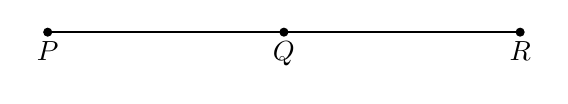
\begin{tikzpicture}
        \draw [-, thick] (0,0)--(6,0);
        \draw [fill] (0,0) circle [radius=0.05] node[below]{$P$};
        \draw [fill] (6,0) circle [radius=0.05] node[below]{$R$};
        \draw [fill] (3,0) circle [radius=0.05] node[below]{$Q$};
      \end{tikzpicture}
      \end{flushright}
      \vspace{1cm}
      \begin{enumerate}
        \item Write a geometric equation: \rule{4cm}{0.15mm} \hspace{1cm} \rule{4cm}{0.15mm}
        \vspace{.7cm}
        \item Substitute algebraic values: \rule{4cm}{0.15mm}
        \item Solve for $x$
        \vspace{4.5cm}
        %\begin{center} $x=$ \rule{1cm}{0.15mm} \end{center}
        \item Answer the question:
        \vspace{2.5cm}
        \item Check your answer
      \end{enumerate}

\end{enumerate}

\end{document}
